\section{Containers}\label{sec:containersimpl}

\subsection{Images}\label{subsec:containersimagesDefinition}
The construction of each of the project's containers was done from a DockerFile in each of the repositories. The DockerFile is a text file that contains all the commands a user can call on the command line to assemble an image. Using the \texttt{docker build} command, the DockerFile is processed and the resulting image is created. The resulting image is a read-only image that can be used to start Docker containers.

For the construction of the database container, a ready-made MongoDB image available on Docker HUB \cite{dockerMongo} was used (Docker platform that serves as a repository of images that can be used for container construction \cite{dockerHub}).

For the construction of the image that contains the API and the Data Reception Module, the image with the Database Initialization, and the image with the Processing Module, a Python image \cite{dockerPython} was used as a base. Subsequently, a script was executed that installs the necessary dependencies and starts the system. %The DockerFile that assembles these images is in the appendices. API and Data Reception Module \ref{apiDockerfile}, Database Initialization \ref{databaseInitializationDockerfile}, and Data Processing Module \ref{processDockerfile}.

For the construction of the container with the Frontend, a Node image \cite{dockerNode} was used as a base, dependencies were installed according to the package manager, then the application was built, and finally, the application was executed. %The DockerFile that assembles this image is in the appendices \ref{frontendDockerfile}.

Lastly, for the construction of the web server, a ready-made NGINX image \cite{dockerNginx} was used with access to volumes that store the server configuration file and necessary Let's Encrypt settings, and exposing ports 80 and 443 for external connections. In addition, for the proper configuration of Let's Encrypt, a container was built with the \texttt{certbot} image \cite{dockerCertbot}, so that it was possible to configure and update the SSL certificate automatically.

\subsection{Docker Compose}\label{subsec:containerscompose}

Given that the project is composed of several containers, Docker Compose was used to facilitate the simultaneous execution of all containers. Docker Compose is a tool for defining and running multi-container Docker applications. With Compose, it is possible to use a YAML file to configure the application's services. Then, with a single command, you can create and start all services from the configuration.

Figure \ref{fig:containersDependencyImpl} shows the containers used to run the system and the dependencies between them.

\begin{figure}[htbp]
	\centering
	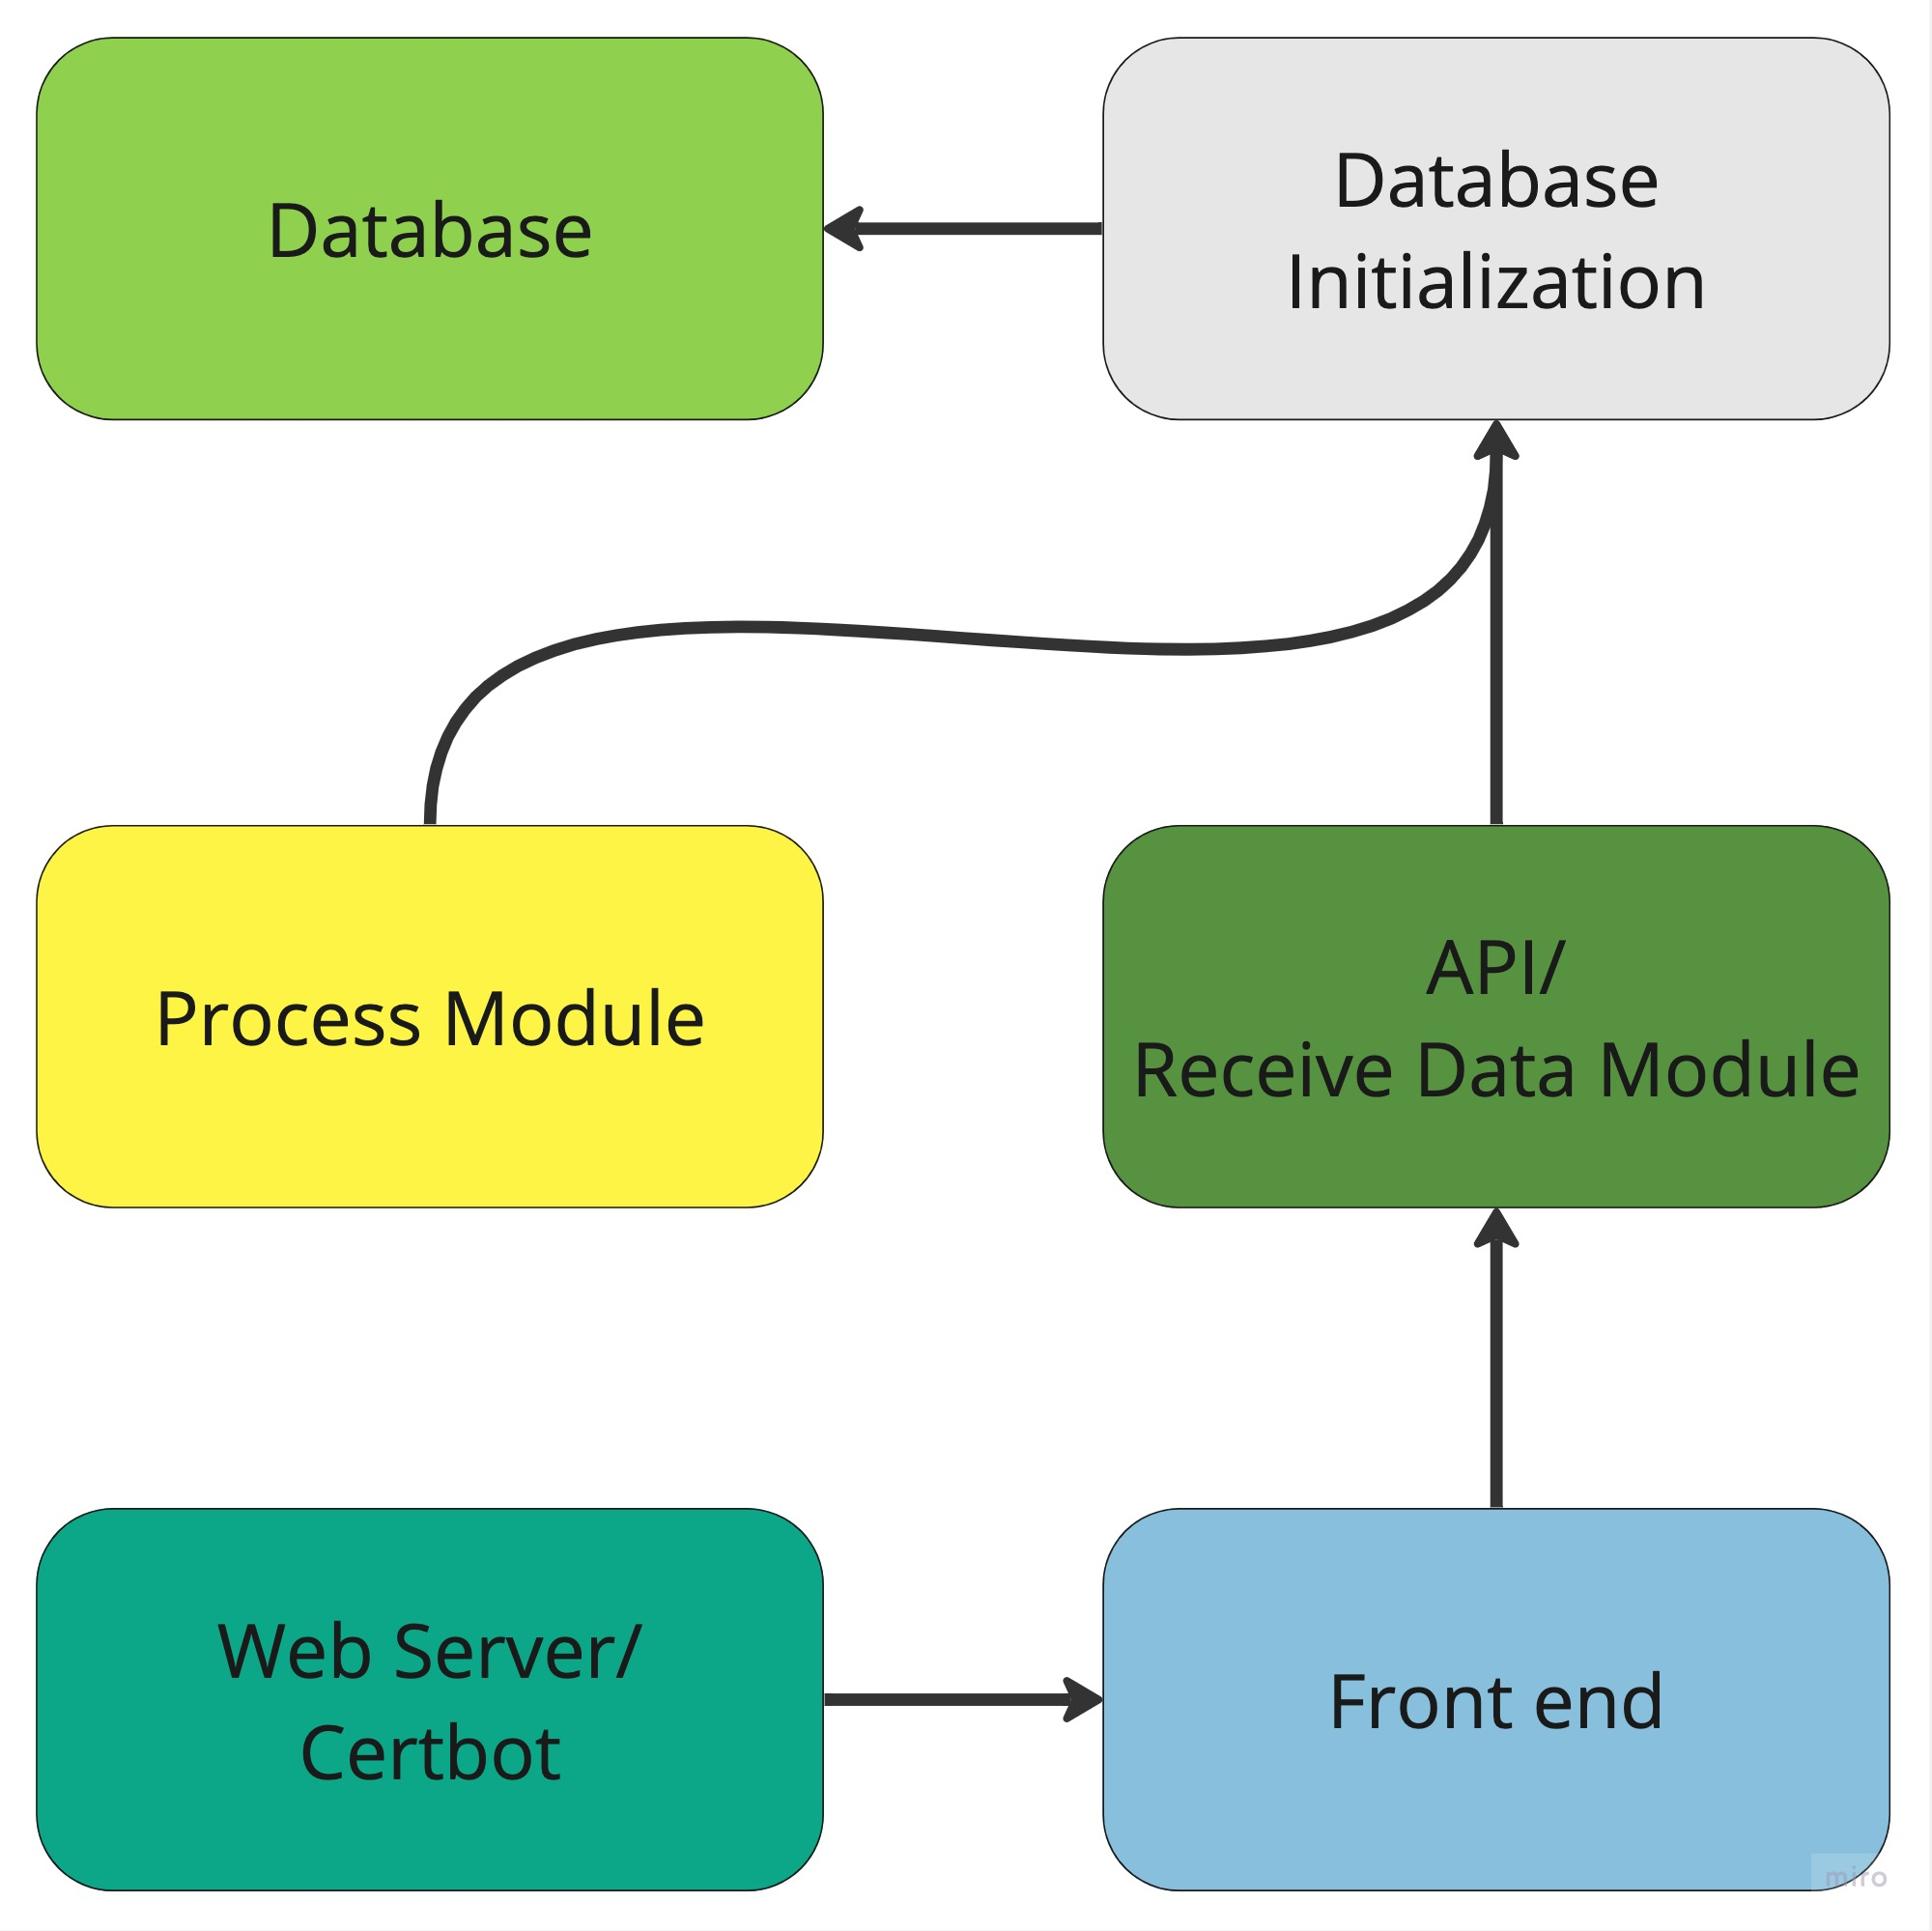
\includegraphics[scale=0.09]{images/containersDependency.jpg}
	\caption{Containers dependency.}
	\label{fig:containersDependencyImpl}
\end{figure}


The Database container uses the MongoDB image to store the project's data. It is configured with root user credentials and mounts the persistent volume \texttt{mongodb\_data\_container} for data storage.

The Database Initialization container is responsible for the initialization and potential population of the database. This container directly depends on the database container to perform its tasks. It uses a custom image, explained in \ref{subsec:containersimagesDefinition}, for this purpose.

The API and data reception module container exposes an API on port 8000. It depends on the database initialization container and connects to the database container using the connection string provided by the internal Docker network.

The data processing module container connects to the database and starts after the Database Initialization container.

The Frontend container directly depends on the API, using the image explained in \label{subsec:containersimages}.

For the container that manages the Web Server using the NGINX image, a periodic restart configuration is made, enabling the SSL certificate to be automatically renewed. It depends on the frontend to start, ensuring that the user interface is available when the server is running.

For the execution of the Web Server, an auxiliary container is used, responsible for the renewal of SSL certificates through \texttt{Certbot} \cite{dockerCertbot}. It is configured to renew the certificates periodically and depends on the frontend, ensuring that the certificate is renewed only when the user interface is available.

The definition of the volume used by the database is explicitly made in the \texttt{Docker Compose} file, which is used by the MongoDB container to store data persistently. The network used by the containers is implicitly defined by Docker Compose, which creates a network for the containers and connects them to it, enabling communication between the containers that make up the system.

%The \texttt{docker-compose.yml} file that defines the configuration of the containers is in the appendices \ref{containerscompose}.